\chapter{Temperature, Entropy, and Equilibrium Distributions}

This lecture proceeds in an order that is at first a little surprising, but finally very natural. We begin not by defining temperature, but by stripping away the human units that obscure it. Only after temperature has been recast as an energy variable, and entropy as a dimensionless quantity, do we turn to equilibrium probabilities, the family \(P(i,E)\), and the derivative relation that deserves to be called temperature. These notes follow Leonard Susskind's Lecture 2 closely; the preserved board figures are kept as documentary evidence, and the chapter also retains curated lecture images prepared with the help of LazyingArt LLC and Video2Book.

\section{Units, Boltzmann's Constant, and the Meaning of Temperature}

The lecture opens with a warning: Boltzmann's constant is not a mysterious extra ingredient of nature. It is, in the first instance, a conversion factor. In that respect it plays the same sort of role as the speed of light when one uses \(c\) to convert between units of length and units of time. Temperature, as it is ordinarily measured, comes in human units. Physics, however, wants to treat it in more fundamental ones.

The human temperature scales are historical constructions. Kelvin is tied to absolute zero, Celsius to the freezing and boiling points of water, and the size of a degree is fixed by convenience rather than by microscopic physics. None of that is wrong, but it does mean that the degree is not the natural unit that statistical mechanics would have chosen if it had been invented from the atom upward.

What then is the natural unit? The lecture insists on a simple answer: temperature is really a measure of energy.

A quick physical example makes the point. In a dilute gas the temperature controls the typical kinetic energy of a molecule. One may write
\begin{equation}
\langle E_{\mathrm{kin}}\rangle = \frac{3}{2}k_B T_{\mathrm{Kelvin}}.
\end{equation}
The factor of \(3\) comes from the three spatial directions, and the factor of \(1/2\) is just the familiar normalization of kinetic energy. What matters for us is that the combination \(k_B T_{\mathrm{Kelvin}}\) has units of energy.

The lecture makes this vivid with a deliberately odd comparison. Put a bowling ball into a fluid in thermal equilibrium. Its speed will be far smaller than that of a molecule, but its characteristic kinetic energy is set by the same temperature. Equal temperature does not mean equal velocity; it means equal energy scale.

For that reason it is natural to absorb the conversion factor into the temperature itself:
\begin{equation}
T := k_B T_{\mathrm{Kelvin}}.
\end{equation}
Now temperature is measured directly in energy units, and the kinetic-energy relation becomes
\begin{equation}
\langle E_{\mathrm{kin}}\rangle = \frac{3}{2}T.
\end{equation}

This is the first real payoff of the lecture. Once we adopt the fundamental temperature \(T\), the Boltzmann constant disappears from the later formulas. It has not ceased to exist; it has merely been absorbed into the units.

\section{Entropy in Human Units and Fundamental Units}

The same cleanup must be performed for entropy. Historically, entropy first appeared in thermodynamics before its microscopic origin was understood. In that setting it carried engineering units, namely energy divided by temperature. If temperature is measured in Kelvin, Carnot's entropy is measured in joules per Kelvin.

From the statistical point of view, however, entropy is built from a probability distribution:
\begin{equation}
S = -\sum_i p_i \log p_i.
\end{equation}
This expression is dimensionless. It is an information-like quantity. When one says that one bit corresponds to \(\log 2\), one is already speaking in that dimensionless language.

The lecture therefore distinguishes carefully between the thermodynamic entropy used in engineering and the dimensionless Boltzmann entropy used in statistical mechanics. Their relation is
\begin{equation}
S = \frac{1}{k_B} S_{\mathrm{Carnot}},
\end{equation}
or equivalently
\begin{equation}
S_{\mathrm{Carnot}} = k_B S.
\end{equation}

There is a simple moral here. Once temperature is measured in energy units and entropy is measured as the dimensionless quantity \(-\sum p\log p\), one may work without explicit factors of \(k_B\). If at some later stage one wishes to return to human units, the conversion can be restored.

\begin{remark}
From this point onward we shall write \(T\) for temperature in energy units and \(S\) for dimensionless statistical entropy. This is exactly the convention the lecture is trying to enforce before the real definition of temperature is given.
\end{remark}

\section{Thermal Equilibrium and the Average Energy}

Only now does the lecture turn to the actual question: what is temperature?

The answer begins with thermal equilibrium. A system in contact with an environment does not, in equilibrium, settle into one exact microscopic state forever. Rather, it fluctuates. Energy passes back and forth between the system and its surroundings, but on the average the macroscopic situation remains stationary. This is the natural setting in which probability enters.

Let us label the microscopic states by \(i\), and let the corresponding energies be \(E_i\). In equilibrium there is a probability \(P(i)\) that the system occupies the \(i\)-th state. These probabilities satisfy the normalization condition
\begin{equation}
\sum_i P(i)=1,
\end{equation}
and the average energy is defined by
\begin{equation}
\sum_i P(i) E_i = E.
\end{equation}
On the board the same quantity is written as \(\langle E\rangle\); later, once the one-parameter family is introduced, it is more convenient to write simply \(E\) for the average energy parameter.

\begin{figure}[t]
\centering

\includegraphics[width=0.78\textwidth]{lecture_02_figure_02.png}
\caption{Normalization and average energy as they appear on the board. The notation on the board drifts slightly between \(E_i\), \(E(i)\), and \(\langle E\rangle\), but the mathematical content is clear.}
\end{figure}

The point of the definition is worth stating carefully. The system's instantaneous energy is not fixed. If it is exchanging energy with a heat bath, a measurement at one time may give one result and a measurement at another time a different one. The equilibrium quantity is the average energy, not a sharply fixed value at every instant.

In the language of the lecture, the outside world that stabilizes the equilibrium is the \emph{heat bath}. This is not yet a full derivation of equilibrium statistical mechanics; it is the setting in which the later definition of temperature becomes meaningful.

\section{A One-Parameter Family of Equilibrium Distributions}

The next move is the decisive one. Equilibrium is not represented by a single probability distribution, but by a family of them. If the average energy is changed, the equilibrium distribution changes with it. Thus one should think in terms of a one-parameter family
\begin{equation}
P(i,E),
\end{equation}
where \(E\) now denotes the average energy labeling the distribution, not the microscopic state energy \(E_i\).

For each value of this parameter, the probabilities are normalized and have the prescribed mean energy:
\begin{align}
\sum_i P(i,E) &= 1, \\
\sum_i P(i,E)\,E_i &= E.
\end{align}
These are the clean equations the notes should use. On the board, the earlier unparameterized formulas remain visible for a while, but the spoken discussion has already moved to the family \(P(i,E)\).

\begin{figure}[t]
\centering

\includegraphics[width=0.88\textwidth]{lecture_02_figure_03.png}
\caption{The board at the moment the graph \(P(i,E)\) is introduced. The left side still carries the normalization and average-energy formulas; the right side opens the new graphical language.}
\end{figure}

The lecture immediately translates this idea into a picture. The horizontal axis can first be thought of as the state label \(i\), but once the states are ordered in increasing energy it may equally well be read as a proxy for the state energy \(E_i\). The vertical axis is the probability distribution.

\begin{figure}[t]
\centering
\begin{tikzpicture}[scale=0.95]
\draw[->] (0,0) -- (0,3.2) node[left] {$P(i,E)$};
\draw[->] (0,0) -- (7.0,0) node[right] {$i$};
\end{tikzpicture}
\caption{A clean reconstruction of the first graph: at this stage the lecture allows the horizontal axis to be read either as the state label \(i\) or, after ordering the states, as the energy of the \(i\)-th state.}
\end{figure}

The mathematical claim is still provisional. The lecture is not yet deriving the Boltzmann distribution. It is only asserting, as a matter of experience, that for each value of the average energy there is an equilibrium probability distribution attached to the system.

\subsection{Question \& Answer}

\paragraph{Question.} Is this not circular? The average energy is computed from the probability distribution, but the probability distribution is being labeled by the average energy.

\paragraph{Answer.} The lecture's answer is intentionally modest. For the moment we simply assume that there exists a one-parameter family of equilibrium distributions. We then discover, for each member of the family, its average energy. Since no two members are assumed to have the same average energy, the average energy can be used as a label for the family. The notation \(P(i,E)\) is therefore a naming convention for a family already assumed to exist; it is not yet a derivation of that family.

A related clarification also matters. The lecture says \emph{average} energy rather than \emph{total} energy because the system under discussion is imagined to be exchanging energy with a heat bath. Its energy fluctuates. The average is the stable quantity.

There is also a brief classroom discussion of degeneracy and labeling. To keep the picture simple, the lecture takes as a working assumption that the states can be ordered by increasing energy and that exact degeneracies may be ignored for now.

\section{Entropy as a Function of the Average Energy}

Once the family \(P(i,E)\) is granted, each member of the family carries its own entropy. Therefore entropy becomes a function of the average energy:
\begin{equation}
S(E) = -\sum_i P(i,E)\log P(i,E).
\end{equation}

This is not yet a universal formula independent of the system. Different systems have different families \(P(i,E)\), so they have different functions \(S(E)\). What matters is that the lecture has now constructed a relation between entropy and energy.

At this point the board picture becomes more informative. As the average energy increases, the distribution spreads and shifts toward larger values of the horizontal variable. Since the occupied region in state space broadens, the entropy also tends to increase.

\begin{figure}[t]
\centering

\includegraphics[width=0.88\textwidth]{lecture_02_figure_04.png}
\caption{The family of distributions after the graph has been developed. The left side still preserves the earlier equilibrium constraints, while the right side makes visible the shift of probability weight toward higher-energy states.}
\end{figure}

\begin{figure}[t]
\centering
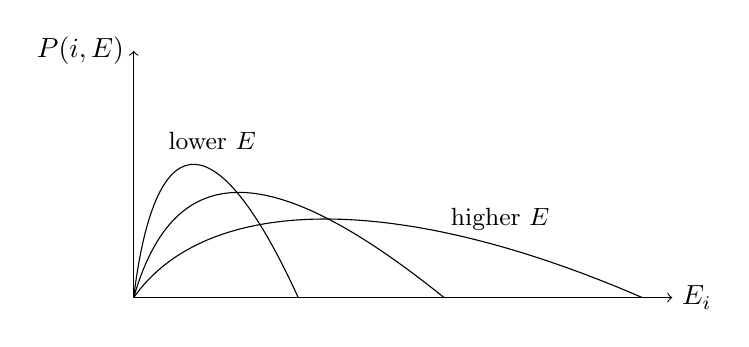
\begin{tikzpicture}[scale=0.95]
\draw[->] (0,0) -- (0,3.3) node[left] {$P(i,E)$};
\draw[->] (0,0) -- (7.2,0) node[right] {$E_i$};

\draw (0,0) .. controls (0.30,2.45) and (1.15,2.30) .. (2.20,0);
\draw (0,0) .. controls (0.55,1.90) and (1.85,1.85) .. (4.15,0);
\draw (0,0) .. controls (0.95,1.35) and (3.45,1.45) .. (6.80,0);

\node at (1.05,2.10) {\small lower \(E\)};
\node at (4.90,1.05) {\small higher \(E\)};
\end{tikzpicture}
\caption{A cleaned schematic of the family \(P(i,E)\). The lecture does not yet calculate these distributions; it uses them as a guided picture for how larger average energy pushes probability toward higher-energy states.}
\end{figure}

The lecture is careful not to overclaim. It takes as a working assumption that, in ordinary physical systems, increasing the average energy tends to spread the distribution over more states and hence tends to increase the entropy. That monotonicity will later justify differentiating one with respect to the other.

\section{Temperature as the Derivative \texorpdfstring{$dE/dS$}{dE/dS}}

We now reach the central mathematical question of the lecture. Suppose we move from one member of the family \(P(i,E)\) to a nearby one. How much energy must be added to change the entropy by a small amount, say by one bit?

The lecture first presents the answer almost as a disappointment. It is only a differential identity:
\begin{equation}
dE = \frac{dE}{dS}\,dS.
\end{equation}
Equivalently,
\begin{equation}
dS = \frac{dS}{dE}\,dE.
\end{equation}
But this seemingly trivial relation hides the important object. The derivative \(dE/dS\) is \emph{temperature}.

\begin{definition}
Temperature is defined by
\begin{equation}
T := \frac{dE}{dS},
\end{equation}
or, equivalently,
\begin{equation}
dE = T\,dS.
\end{equation}
One may also write
\begin{equation}
dS = \frac{1}{T}\,dE.
\end{equation}
\end{definition}

This is the universal definition the lecture wants to isolate. Temperature is not introduced first as a sensory notion and only later ornamented with formulas. It is introduced directly as the energy cost of a small entropy increase.

If one wants to change the entropy by one bit, then \(dS\) should be read as \(\log 2\), at least heuristically. The corresponding energy change is then approximately \(T\log 2\) when the variation is small enough that \(T\) may be treated locally as constant. This is a useful mental picture even though the lecture immediately returns to the differential form.

There is also a pleasant consistency check with the earlier discussion of units. Since
\begin{equation}
T = k_B T_{\mathrm{Kelvin}}, \qquad S = \frac{1}{k_B}S_{\mathrm{Carnot}},
\end{equation}
substituting these into \(dE=T\,dS\) gives
\begin{equation}
dE = T_{\mathrm{Kelvin}}\, dS_{\mathrm{Carnot}}.
\end{equation}
The \(k_B\) factors cancel. Thus the thermodynamic relation has the same form in human units and in fundamental units.

\section{Two Weakly Coupled Systems and the Direction of Energy Flow}

A definition is not enough. The lecture wants to recover the ordinary physical meaning of temperature: when two systems are brought into weak contact, which way does energy flow?

Consider two systems \(A\) and \(B\), each initially in equilibrium, and let them exchange only small amounts of energy. The lecture represents this by connecting them with a thin pipe. The coupling is weak enough that the individual thermodynamic descriptions remain meaningful, but strong enough that energy can pass back and forth.

Now assume that initially \(T_B > T_A\). We want to show that energy flows from \(B\) to \(A\).

Three ingredients are assembled on the board.

First, entropy is additive:
\begin{equation}
S_{\mathrm{tot}} = S_A + S_B.
\end{equation}

Second, total energy is conserved:
\begin{equation}
dE_A = -\,dE_B.
\end{equation}

Third, the second law states that the total entropy increases during equilibration:
\begin{equation}
dS_A + dS_B > 0.
\end{equation}

Using the definition of temperature for each subsystem,
\begin{equation}
dE_A = T_A\, dS_A, \qquad dE_B = T_B\, dS_B,
\end{equation}
we may rewrite the entropy changes as
\begin{equation}
dS_A = \frac{dE_A}{T_A}, \qquad dS_B = \frac{dE_B}{T_B}.
\end{equation}
Therefore
\begin{align}
dS_{\mathrm{tot}}
  &= dS_A + dS_B \\
  &= \frac{dE_A}{T_A} + \frac{dE_B}{T_B} \\
  &= \frac{dE_A}{T_A} - \frac{dE_A}{T_B} \\
  &= dE_A\left(\frac{1}{T_A}-\frac{1}{T_B}\right).
\end{align}

Now if \(T_B>T_A\), then
\begin{equation}
\frac{1}{T_A}-\frac{1}{T_B} > 0.
\end{equation}
The second law requires \(dS_{\mathrm{tot}}>0\), and therefore we must have
\begin{equation}
dE_A > 0.
\end{equation}
So system \(A\) gains energy while system \(B\) loses it. Energy flows from the hotter system to the colder system.

\begin{remark}
The lecture transcript breaks off while this algebra is being assembled, but the completion above uses only the equations that have already been explicitly stated on the board and in the spoken argument.
\end{remark}

This is the point at which the abstract definition of temperature becomes operational. Temperature is the quantity that decides the direction of spontaneous energy flow.

\section{Summary}

The lecture begins by clearing away a notational obstacle. Temperature in its natural form is an energy, and entropy in its natural form is dimensionless. Once that is understood, equilibrium is described by probabilities \(P(i)\), then by a one-parameter family \(P(i,E)\), and finally by an entropy function \(S(E)\).

From that family one extracts the defining derivative
\[
T=\frac{dE}{dS},
\]
or \(dE=T\,dS\). Temperature is thus the energy price of a small entropy change. When two systems are weakly coupled, this same derivative controls the direction of energy flow: energy passes from the larger value of \(T\) to the smaller one. In that sense the lecture rebuilds the ordinary notion of hot and cold from probability, entropy, and energy alone.